% Autoencoder neural networks are a type of deep learning algorithm that has shown great potential in data compression, noise reduction, and feature extraction. When applied to digital cryptography, autoencoder neural networks can be used to encrypt and decrypt sensitive data in a more secure and efficient way by creating highly complex and unique encryption keys that are difficult to predict or duplicate, making them more resistant to attacks.


% This is my introduction \cite{icaart20}.

\subsection{Cryptography}

Cryptography is the study of techniques for secure communication, so that third parties cannot read messages sent between the sender and the receiver. An encryption algorithm is a mathematical function that transforms a message into a form that is difficult to predict or duplicate. Several encryption methods have been developed over the years, the most popular and widely used involve the use of a key, which defines how the message is encoded and decoded, for example, the Advanced Encryption Standard (AES) \cite{aes}. Cryptography has many applications, such as authentication, confidentiality, integrity, and non-repudiation.

\subsection{Autoencoder Neural Networks}

Autoencoders are a type of neural networks whose purpose is to learn efficient representations of data by undergoing unsupervised training \cite{autoencoder}. When training an autoencoder, the network learns to reconstruct the original data by encoding the information in a latent space, which is a representation that captures the essential features of the data. These neural networks have a symmetric architecture, in other words, their input is the same shape as their output, and the middle layer is the one responsible for the representation of the data. The middle layer is usually called the code layer.

Autoencoder neural networks are used in tasks such as dimensionality reduction, anomaly detection, signal processing, data compression, and cryptography.

\begin{figure}[h]
    \centering
    

\tikzset{every picture/.style={line width=0.75pt}} %set default line width to 0.75pt        

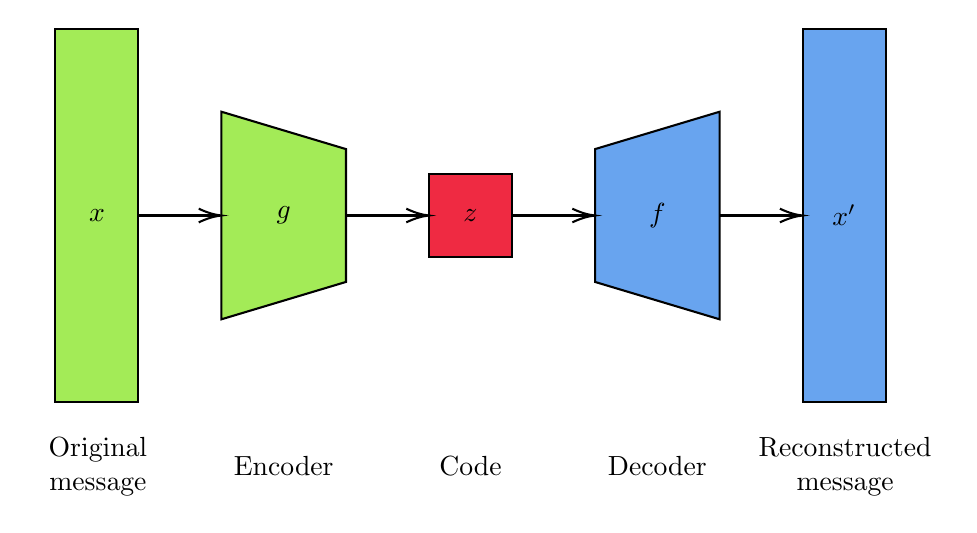
\begin{tikzpicture}[x=0.75pt,y=0.75pt,yscale=-1,xscale=1]
    %uncomment if require: \path (0,300); %set diagram left start at 0, and has height of 300

    %Shape: Rectangle [id:dp8942019960286618] 
    \draw  [fill={rgb, 255:red, 163; green, 235; blue, 87 }  ,fill opacity=1 ] (20,20) -- (60,20) -- (60,200) -- (20,200) -- cycle ;
    %Shape: Trapezoid [id:dp4630434446283549] 
    \draw  [fill={rgb, 255:red, 163; green, 235; blue, 87 }  ,fill opacity=1 ] (100,60) -- (160,78) -- (160,142) -- (100,160) -- cycle ;
    %Shape: Rectangle [id:dp7342042996288556] 
    \draw  [fill={rgb, 255:red, 239; green, 42; blue, 66 }  ,fill opacity=1 ] (200,90) -- (240,90) -- (240,130) -- (200,130) -- cycle ;
    %Shape: Trapezoid [id:dp8342225116725475] 
    \draw  [fill={rgb, 255:red, 104; green, 164; blue, 239 }  ,fill opacity=1 ] (340,60) -- (280,78) -- (280,142) -- (340,160) -- cycle ;
    %Shape: Rectangle [id:dp23031828799634058] 
    \draw  [fill={rgb, 255:red, 104; green, 164; blue, 239 }  ,fill opacity=1 ] (380,20) -- (420,20) -- (420,200) -- (380,200) -- cycle ;
    %Straight Lines [id:da7729793473503881] 
    \draw    (60,110) -- (98,110) ;
    \draw [shift={(100,110)}, rotate = 180] [color={rgb, 255:red, 0; green, 0; blue, 0 }  ][line width=0.75]    (10.93,-3.29) .. controls (6.95,-1.4) and (3.31,-0.3) .. (0,0) .. controls (3.31,0.3) and (6.95,1.4) .. (10.93,3.29)   ;
    %Straight Lines [id:da237260655681939] 
    \draw    (160,110) -- (198,110) ;
    \draw [shift={(200,110)}, rotate = 180] [color={rgb, 255:red, 0; green, 0; blue, 0 }  ][line width=0.75]    (10.93,-3.29) .. controls (6.95,-1.4) and (3.31,-0.3) .. (0,0) .. controls (3.31,0.3) and (6.95,1.4) .. (10.93,3.29)   ;
    %Straight Lines [id:da21321769920852573] 
    \draw    (240,110) -- (278,110) ;
    \draw [shift={(280,110)}, rotate = 180] [color={rgb, 255:red, 0; green, 0; blue, 0 }  ][line width=0.75]    (10.93,-3.29) .. controls (6.95,-1.4) and (3.31,-0.3) .. (0,0) .. controls (3.31,0.3) and (6.95,1.4) .. (10.93,3.29)   ;
    %Straight Lines [id:da5140682018274638] 
    \draw    (340,110) -- (378,110) ;
    \draw [shift={(380,110)}, rotate = 180] [color={rgb, 255:red, 0; green, 0; blue, 0 }  ][line width=0.75]    (10.93,-3.29) .. controls (6.95,-1.4) and (3.31,-0.3) .. (0,0) .. controls (3.31,0.3) and (6.95,1.4) .. (10.93,3.29)   ;

    % Text Node
    \draw (40.5,231) node   [align=left] {\begin{minipage}[lt]{44.12pt}\setlength\topsep{0pt}
            \begin{center}
                Original\\message
            \end{center}

        \end{minipage}};
    % Text Node
    \draw (400.5,231) node   [align=left] {\begin{minipage}[lt]{68.49pt}\setlength\topsep{0pt}
            \begin{center}
                Reconstructed\\message
            \end{center}

        \end{minipage}};
    % Text Node
    \draw (130,230.5) node   [align=left] {\begin{minipage}[lt]{40.72pt}\setlength\topsep{0pt}
            \begin{center}
                Encoder
            \end{center}

        \end{minipage}};
    % Text Node
    \draw (310,230.5) node   [align=left] {\begin{minipage}[lt]{41.28pt}\setlength\topsep{0pt}
            \begin{center}
                Decoder
            \end{center}

        \end{minipage}};
    % Text Node
    \draw (220,230.5) node   [align=left] {\begin{minipage}[lt]{27.1pt}\setlength\topsep{0pt}
            \begin{center}
                Code
            \end{center}

        \end{minipage}};
    % Text Node
    \draw (40,110) node    {$x$};
    % Text Node
    \draw (130,110) node    {$g$};
    % Text Node
    \draw (220,110) node    {$z$};
    % Text Node
    \draw (310,110) node    {$f$};
    % Text Node
    \draw (400,110) node    {$x'$};


\end{tikzpicture}
    \caption{Autoencoder neural network.}
    \label{fig:autoencoder}
\end{figure}

A basic autoencoder architecture is shown in \ref{fig:autoencoder}. The autoencoder may be expressed in mathematical terms as follows:
%
\begin{equation}\label{eq:autoencoder}
    \begin{split}
        z &= g(x) \\
        x' &= f(z) \\
        x &\approx x' \\
    \end{split}
\end{equation}
%
where $x$ is the input, $z$ is the code, $x'$ is the output, $g$ is the encoder, and $f$ is the decoder.
